\section{Cartographie applicative cible et prototype}
\label{sec:applicatif}

\subsection{Composants applicatifs}
La cartographie applicative (figure~\ref{fig:applicatif}) traduit les blocs fonctionnels en quinze composants logiciels, regroupés en sept quartiers~: canaux, identité numérique, orchestration et services d'IA, cœur métier, support et données, intégration, et systèmes externes. Le choix structurant est l'introduction d'un \textbf{moteur de processus} (APP-04) qui orchestre la demande de bout en bout et porte les règles de routage~; les canaux ne contiennent plus de logique métier et les services d'IA sont des composants autonomes, appelés par le moteur, remplaçables indépendamment. Une \textbf{passerelle d'API} (APP-11) centralise les échanges avec l'état civil, la Trésorerie, Barid Al-Maghrib et les consulats, ce qui supprime les interfaces point à point.

\begin{figure*}[t]
\centering
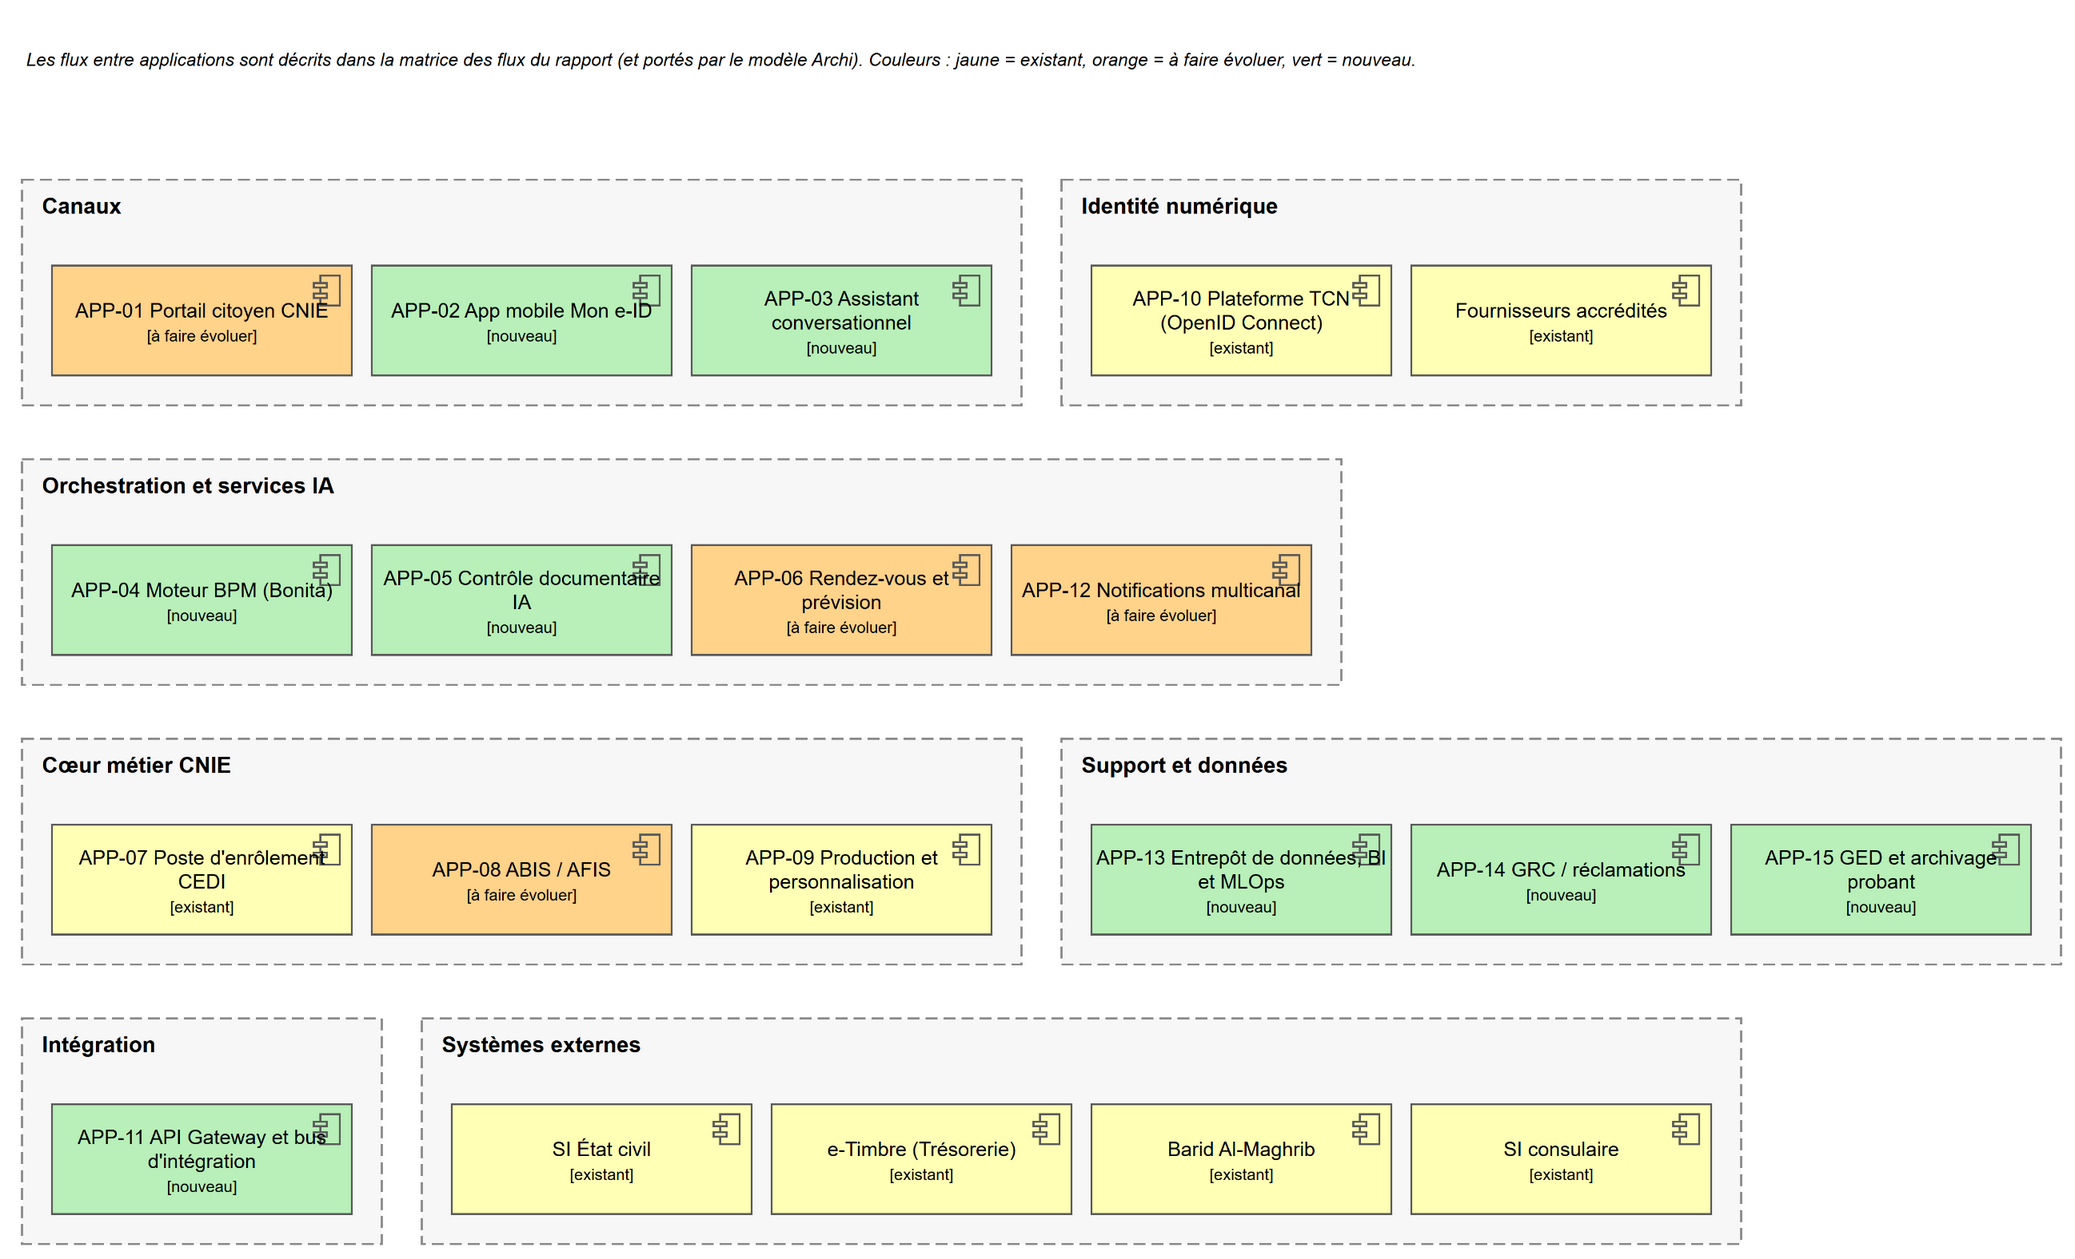
\includegraphics[width=0.98\textwidth]{archimate/V4_applicatif.png}
\caption{Cartographie applicative cible~: quinze composants et cinq systèmes externes, avec leur statut.}
\label{fig:applicatif}
\end{figure*}

\subsection{Matrice des flux}
Le tableau~\ref{tab:flux} décrit les principaux flux entre composants. Tous transitent par le bus d'événements de la zone applicative (publication d'événements de statut) ou par des appels d'API synchrones sécurisés par jetons~; aucune base de données n'est partagée entre deux composants.

\begin{table}[h]
\caption{Principaux flux applicatifs cibles}
\label{tab:flux}
\centering
\small
\begin{tabularx}{\columnwidth}{llX}
\toprule
\textbf{Source} & \textbf{Cible} & \textbf{Contenu du flux} \\
\midrule
APP-01 / 02 & APP-04 & Création et mise à jour de la demande, pièces téléversées \\
APP-10 & APP-01 / 02 & Authentification du citoyen (OpenID Connect), attributs d'identité après consentement \\
APP-03 & APP-01 / 02 & Réponses de l'assistant, aide contextuelle à la saisie \\
APP-04 & APP-05 & Pièces à contrôler~; retour du score de conformité et des anomalies \\
APP-04 & APP-06 & Demande de créneaux~; retour des créneaux recommandés \\
APP-04 & APP-11 & Vérification de l'e-timbre, récupération de l'acte d'état civil, ordre de livraison \\
APP-04 & APP-07 & Convocation (QR code) et dossier pré-qualifié \\
APP-07 & APP-08 & Gabarits biométriques pour dédoublonnage et contrôle de fraude \\
APP-08 & APP-09 & Dossier validé pour production \\
APP-09 & APP-04 & Événements de statut (en production, disponible, expédiée) \\
APP-04 & APP-12 & Événements à notifier (SMS, e-mail, notification mobile) \\
APP-04 / 06 / 09 & APP-13 & Journal d'événements anonymisé pour la BI et l'entraînement des modèles \\
APP-04 / 09 & APP-15 & Pièces et récépissés à archiver avec horodatage \\
APP-14 & APP-04 & Réclamations rattachées à une demande \\
Fournisseurs & APP-10 & Délégation d'authentification (inchangée) \\
\bottomrule
\end{tabularx}
\end{table}

\subsection{Plateforme d'IA}
Les composants APP-03, APP-05, APP-06 et APP-08 consomment une plateforme d'inférence commune (zone IA de l'architecture technique). Trois choix de conception protègent la DGSN~: les modèles sont hébergés sur site, les données biométriques ne quittent jamais la zone sécurisée, et chaque modèle est versionné dans un registre avec ses métriques de performance et d'équité, suivies par le composant MLOps d'APP-13. L'assistant conversationnel n'accède qu'à une base de connaissances documentaire validée et ne traite aucune donnée d'identité.

\subsection{Prototype Bonita du sous-processus SP1}
Le sous-processus SP1 a été implémenté sous Bonita Studio Community afin de valider l'orchestration, les règles de décision et les interfaces (figure~\ref{fig:bonita-proc}). Le modèle de données métier comprend quatre objets~: \texttt{DemandeCNIE} (identité, état civil, adresse, contact, statut, score), \texttt{PieceJustificative} (type, fichier, verdict de l'IA), \texttt{RendezVous} (centre, date, créneau, QR code) et \texttt{Centre} (capacité et charge prévue). Trois acteurs sont définis~: le citoyen, initiateur du processus~; l'agent instructeur~; et les tâches de service automatiques.

\begin{figure}[h]
\centering
\IfFileExists{figures/bonita/bonita-diagramme.png}{\includegraphics[width=\columnwidth]{bonita/bonita-diagramme.png}}{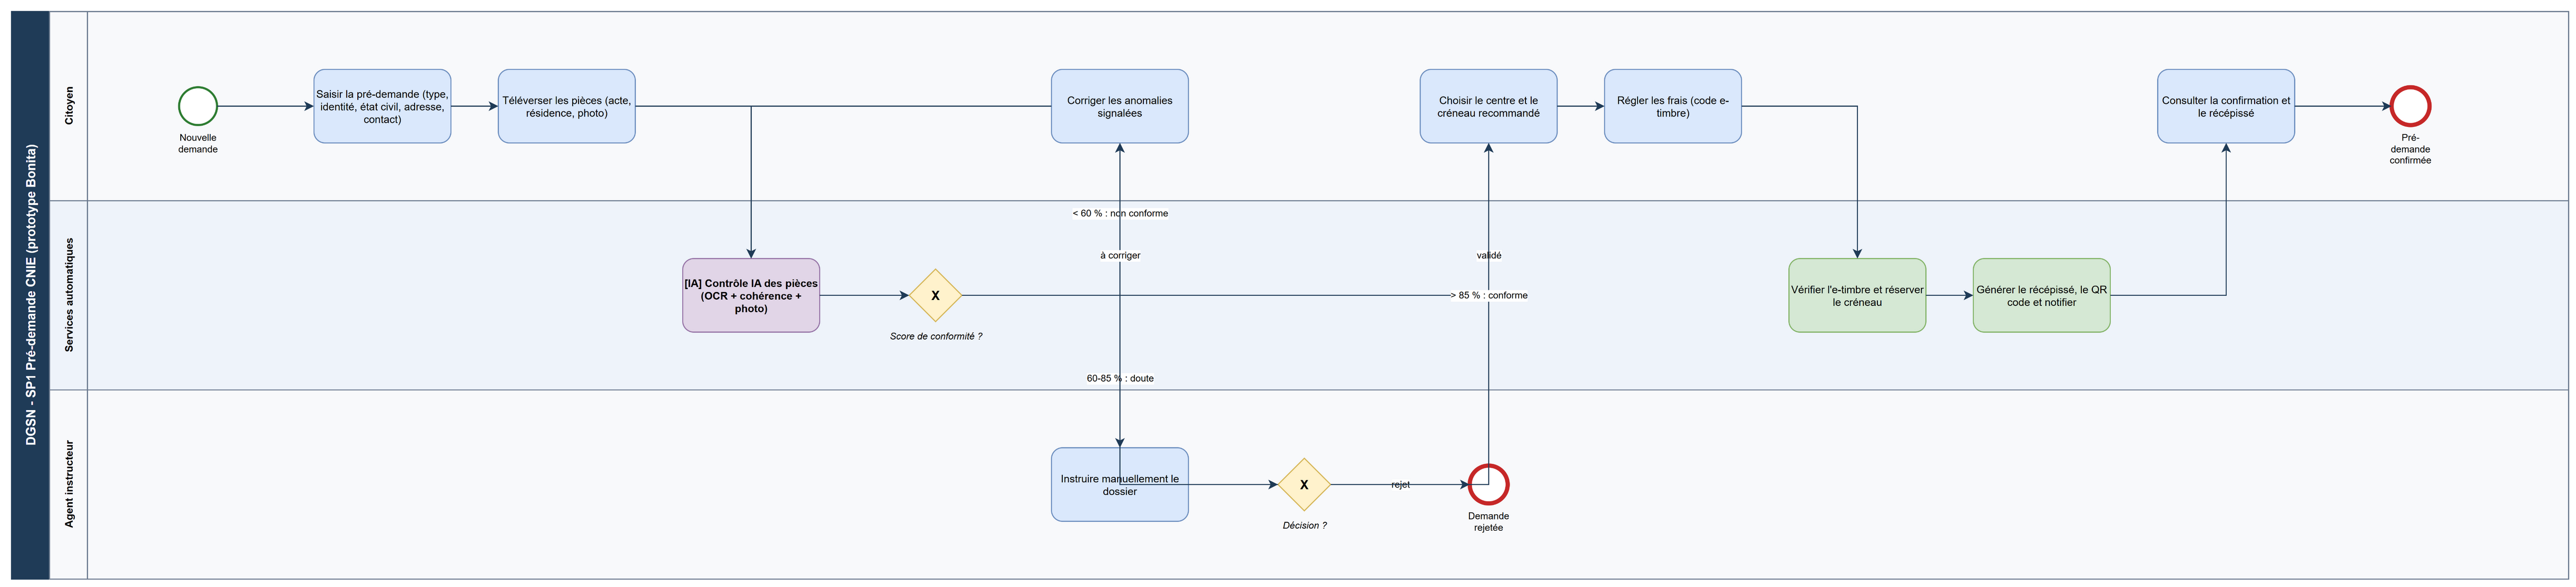
\includegraphics[width=\columnwidth]{bpmn/SP1_predemande_bonita.png}}
\caption{Sous-processus SP1 implémenté sous Bonita~: pré-demande, contrôle des pièces, instruction, rendez-vous et paiement.}
\label{fig:bonita-proc}
\end{figure}

Le parcours comporte six écrans (figure~\ref{fig:bonita-ecrans})~: (1)~saisie de la pré-demande avec validation des formats~; (2)~téléversement des pièces~; (3)~résultat du contrôle automatique sous forme de jauge de conformité et de liste d'anomalies, avec reprise des seules pièces à corriger~; (4)~choix du centre, affichage de sa charge prévue et des créneaux recommandés~; (5)~saisie du code e-timbre~; (6)~confirmation avec numéro de demande et QR code de convocation. Un septième écran, réservé à l'agent instructeur, présente le dossier et les anomalies et recueille sa décision.

Le service de contrôle documentaire est simulé par un connecteur de script qui calcule un score à partir de la présence des pièces et de règles de nommage~; la passerelle exclusive route la demande selon trois seuils (conforme au-delà de 85, instruction humaine entre 60 et 85, correction en deçà). Cette simulation suffit à démontrer la logique du processus~; en production, le connecteur appelle l'API du composant APP-05.

\begin{figure*}[t]
\centering
\IfFileExists{figures/bonita/F1-predemande.png}{%
\begin{subfigure}[t]{0.32\textwidth}\includegraphics[width=\textwidth]{bonita/F1-predemande.png}\caption{Pré-demande}\end{subfigure}\hfill
\begin{subfigure}[t]{0.32\textwidth}\includegraphics[width=\textwidth]{bonita/F3-resultat-ia.png}\caption{Résultat du contrôle IA}\end{subfigure}\hfill
\begin{subfigure}[t]{0.32\textwidth}\includegraphics[width=\textwidth]{bonita/F4-creneau.png}\caption{Créneaux recommandés}\end{subfigure}}{%
\fbox{\parbox{0.9\textwidth}{\centering\vspace{2cm}Captures d'écran des formulaires Bonita (à insérer~: \texttt{figures/bonita/F1-predemande.png}, \texttt{F3-resultat-ia.png}, \texttt{F4-creneau.png})\vspace{2cm}}}}
\caption{Interfaces du prototype Bonita (UI Designer).}
\label{fig:bonita-ecrans}
\end{figure*}
